
\chapter{Introduction : }
	\section{Problématique : }
	\paragraph{Limite des méthodes de recherche CLASSIQUES}
	Bien que les méthodes présentées précédemment (voir \ref{part1})présentent des résultats assez satisfaisant, ils ne permettent pas de résoudre le problème en un temps assez petit, cela nous a conduit à explorer une toute autre famille d'algorithmes appelés les méta-heuristiques.
	\section{Définitions}
	
		\subsection{Espace des solutions}
		\paragraph{}
		L'espace des solutions $S$ d'un problème donné est l'ensemble de toutes les solutions possibles pour ce problème(qu'elles soient positives ou négatives), une solution étant le résultat produit par les méthodes vues dans la partie \ref{part1}
		\begin{figure}[H]
			\centering
			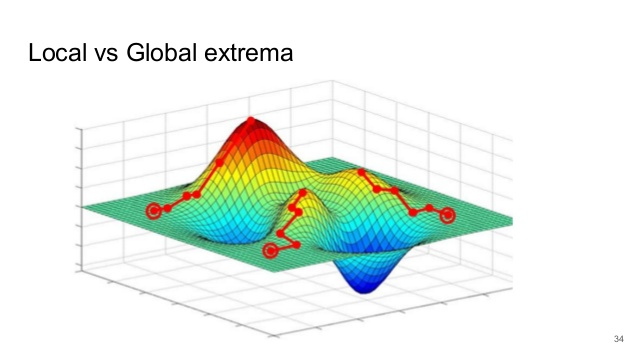
\includegraphics[width=0.75\textwidth]{images/solutionSpace.jpg}
			\caption{Exemple d'un espace de solution multidimensionnel}
		\end{figure}
		\subsection{Métaheuristique}
			\paragraph{}
			Les métaheuristiques sont des algorithmes d'optimisation de solutions visant à résoudre des problèmes hautement combinatoires et dont la complexité ne permet pas leur résolution en un temps raisonnable par des méthodes classiques, elles ont la particularité de faire une recherche dans l'espace $S$ des solutions possibles d'un problème, contrairement aux heuristiques qui construisent les solutions pas à pas en explorant l'espace des états d'une solution en particulier
			\begin{figure}[H]
				\centering
				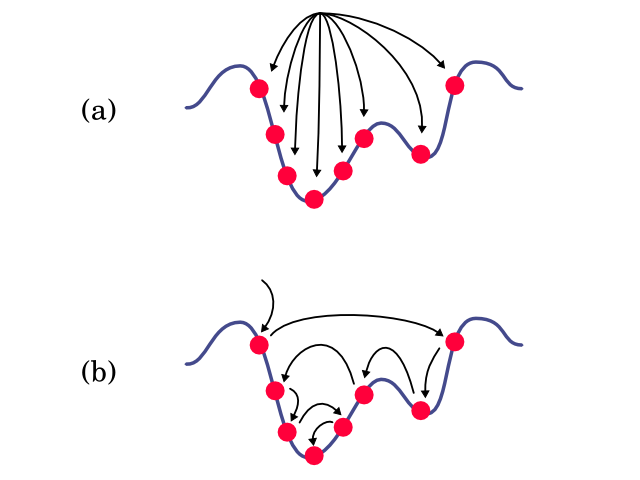
\includegraphics[scale=0.25]{images/metHeur.png}
				\caption{Exemples de recherche ans l'espace des solutions selon une fonction d'évaluation}
			\end{figure}
		\noindent
		\subsection{Intelligence en essaim (Swarm intelligence) }
		\paragraph{}
		L'intelligence en essaim consiste à étudier et à construire des sociétés d'individus artificiels simples qui sont capables collectivement de fournir une réponse complexe et parviennent a travers des interactions(aussi appelés \textbf{synergie}) simples.
		\subsection{Bee swarm optimization (BSO)}
		
		\paragraph{} 
		C'est un algorithme de recherche de solutions à base de populations d'agents artificielles qui imitent le comportement des abeilles dans leur façon de rechercher la nourriture d'une façon organisé et optimale, la nourriture étant l'analogie d'une solution dans le domaine de l'intelligence artificielle(Résolution de problèmes).
		\begin{figure}[H]
			\centering
			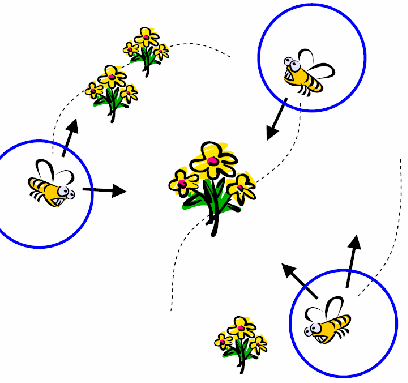
\includegraphics{images/beesSearching.png}
			\caption{Abeilles communiquant pour la recherche de nourriture}
		\end{figure}
		
		